\begin{Problem}
	Betrachten Sie die folgenden Familien von Kraftfeldern auf geeigneten Definitionsbereichen $D_\eta^{(n)}  \subseteq \R^3$
	\begin{align*}
		F_\eta^{(1)}:& D_\eta^{(1)}\ni \va x\to r^\eta\cdot \va x\in \R^3\\
		F_\eta^{(2)}:& D_\eta^{(2)}\ni\va x \to r_{12}^\eta\cdot(x_1\va e_1-x_2\va e_2)\in \R^3\\
		F_\eta^{(3)}:& D_\eta^{(3)}\ni \va x\to r_{12}^\eta\cdot\left( x_2\va e_1-x_1\va e_2 \right) \in\R^3\\
		F_\eta^{(4)}:&D_\eta^{(3)}\ni \va x\to r_{12}^\eta\cdot\left( x_2\va e_1+x_1\va e_2 \right) \in \R^3
	\end{align*}
	wobei $r_{12}=\sqrt{x_1^2+x_2^2} $ und $r=\sqrt{x_1^2+x_2^2+x_3^3} $
	Skizzieren Sie die Felder $\va F_\eta^{(n)}$ als Vektorpfeile in der von den Einheitsvektoren $\va e_1$ und $\va e_2$ aufgespannten Ebene (hier genügt es, zwischen den Fällen $\eta > -1, \eta = -1$ und $\eta < -1$ zu unterscheiden). 
	
	Bestimmen Sie, abhängig von der Potenz $\eta \in \R$,
	\begin{enumerate}
		\item den maximalen Definitionsbereich $D_\eta^{(n)}$,
		\item die maximale Bereiche $C_\eta^{(n)}\subseteq D_\eta^{(n)}$, auf denen $F_\eta^{(n)}$ konservativ ist,
		\item eine Potentialfunktion $V_\eta^{(n)}:C_{\eta}^{(n)}\to \R$ mit $F_\eta^{(n)}=-\grad{V_\eta^{(n)}}$, sofern sie existiert,
		\item das Kurvenintegral
		\[I_\eta^{(n)}(R)=\int_{\gamma_R}\dd{\va\xi}\cdot\va F_\eta^{(n)}(\va\xi)\]
		über den gegen den Uhrzeigersinn umlaufenen Kreis $\gamma_R$ mit Radius $R$ und Mittelpunkt $\va0$ in der von $\va e_1$ und $\va e_2$ aufgespannten Ebene
		\begin{center}
			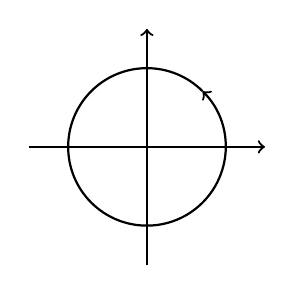
\begin{tikzpicture}
				\draw[thick, ->] (-1.5,0) -- (1.5,0);
				\draw[thick, ->] (0,-1.5) -- (0,1.5);
				\draw[thick, ->] ({1/sqrt(2)},{1/sqrt(2)}) arc (45:405:1);
			\end{tikzpicture}
		\end{center}
	\end{enumerate}
\end{Problem}
